% !TeX root = ../thesis.tex

\begin{translation}
\label{cha:translation}

\newlength{\defaultListTopsep}
\defaultListTopsep=0.25\parskip
\setlist{
	partopsep=0mm,
	topsep=\defaultListTopsep,
	itemsep=0mm,
	parsep=\parskip
}

\newenvironment{displayLinesTable}[1][l]{%
	\par
	\vspace{\defaultListTopsep}%
	\noindent\begin{tabular}{@{\hspace{\leftmargin}}#1}%
}{%
	\end{tabular}\par
	\vspace{\defaultListTopsep}%
	\ignorespacesafterend
}

\newenvironment{commentary}{%
	\vspace{-1.5mm}
	\list{}{
		\topsep		0mm
		\partopsep	0mm
		\listparindent	1.5em
		\itemindent	\listparindent
		\rightmargin	\leftmargin
		\parsep		0mm
	}
	\item
	\small\em
	\noindent\nopagebreak\rule{\linewidth}{1pt}\par
	\noindent\ignorespaces
}{%
	\endlist
}

% New column types to use in tabular environment for instruction formats.
% Allocate 0.18in per bit.
\newcolumntype{I}{>{\centering\arraybackslash}p{0.18in}}
% Two-bit centered column.
\newcolumntype{W}{>{\centering\arraybackslash}p{0.36in}}
% Three-bit centered column.
\newcolumntype{F}{>{\centering\arraybackslash}p{0.54in}}
% Four-bit centered column.
\newcolumntype{Y}{>{\centering\arraybackslash}p{0.72in}}
% Five-bit centered column.
\newcolumntype{R}{>{\centering\arraybackslash}p{0.9in}}
% Six-bit centered column.
\newcolumntype{S}{>{\centering\arraybackslash}p{1.08in}}
% Seven-bit centered column.
\newcolumntype{O}{>{\centering\arraybackslash}p{1.26in}}
% Eight-bit centered column.
\newcolumntype{E}{>{\centering\arraybackslash}p{1.44in}}
% Ten-bit centered column.
\newcolumntype{T}{>{\centering\arraybackslash}p{1.8in}}
% Twelve-bit centered column.
\newcolumntype{M}{>{\centering\arraybackslash}p{2.2in}}
% Sixteen-bit centered column.
\newcolumntype{K}{>{\centering\arraybackslash}p{2.88in}}
% Twenty-bit centered column.
\newcolumntype{U}{>{\centering\arraybackslash}p{3.6in}}
% Twenty-bit centered column.
\newcolumntype{L}{>{\centering\arraybackslash}p{3.6in}}
% Twenty-five-bit centered column.
\newcolumntype{J}{>{\centering\arraybackslash}p{4.5in}}

\newcommand{\instbit}[1]{\mbox{\scriptsize #1}}
\newcommand{\instbitrange}[2]{~\instbit{#1} \hfill \instbit{#2}~}
\newcommand{\reglabel}[1]{\hfill {\tt #1}\hfill\ }

%------------------------------------------------------------------------------
%------------------------------------------------------------------------------

\newcommand{\z}[1]{{\tt\catcode`\`=\active\protect\frenchspacing#1}}
\newcommand{\zSafe}[1]{{\tt #1}}
\newcommand{\LB}{\char123}
\newcommand{\RB}{\char125}
\newcommand{\RISCV}{RISC-V}

\newcommand{\WIRI}{\textbf{WIRI}}
\newcommand{\WPRI}{\textbf{WPRI}}
\newcommand{\WLRL}{\textbf{WLRL}}
\newcommand{\WARL}{\textbf{WARL}}

\newcommand{\unspecified}{\textsc{unspecified}}

\title{RISC-V 高级中断架构(第一章至第三章第六节)}
\maketitle

\tableofcontents

\section{介绍}
\label{ch:intro}

本文档指定了 {\RISCV} 高级中断架构,包括:(a) 对 {\RISCV} 标准特权架构的扩展({\RISCV} 指令集手册第二卷中指定的 Harts);(b) 用于 {\RISCV} 系统的两个标准中断控制器:高级平台级中断控制器 (APLIC, Advanced Platform-Level Interrupt Controller) 和消息驱动中断控制器(IMSIC, Incoming Message-Signaled Interrupt Controller);和 (c) 与中断有关的其他系统部件的要求。

\begin{commentary}
    本章内容主要是关于我们的设计决策,实现选项和应用场景的说明,读者如果只对规范感兴趣,可以跳过这章。
\end{commentary}

\subsection{目标}

{\RISCV} 高级中断架构有以下目标:
\begin{itemize}

\item 以 {\RISCV} 的中断处理功能为基础构建特权架构,最大限度地减少对现有功能的替换。
\item 除了基本的有线中断外,为{\RISCV}系统提供直接使用 PCI Express 和其他设备标准所采用的消息驱动中断(MSIs, message-signaled interrupt)的设施。
\item 对于有线中断,定义一个新的平台级中断控制器 (高级 PLIC 或 APLIC),为每个特权级({\RISCV M 和 S 特权级})提供独立的控制界面,并且可以将有线中断转换为系统支持的消息驱动中断。
\item 在{\RISCV} Hart 上扩展本地中断的框架。
\item 可选地允许软件将所有中断源的相对优先级配置到 {\RISCV} Hart (包括标准的时钟中断和软件中断等),而不是受限于由一个单独的中断控制器处理外部中断的优先级。
\item 当 Hart 实现特权架构的虚拟化扩展时,为虚拟机中断虚拟化提供足够的支持。
\item 借助用于重定向 MSI 的 IOMMU (I/O内存管理单元),最大限度地为客户操作系统提供对设备直接进行控制的能力,同时最小化虚拟机监管程序的参与。
\item 避免虚拟机数量受到中断硬件的限制。
\item 尽可能地权衡速度、效率和灵活性并实现上述所有功能。

\end{itemize}

高级中断架构的最初版本主要针对更大型、高性能的RISCV系统的需求。目前还没有定义对下列以下中断处理特性的支持,这些特性可以在所谓的“实时“系统中减小中断响应时间,但不太适合高速处理器:

\begin{itemize}
\item 给每个中断源一个单独的陷入入口地址;
\item 在陷入时自动保存和恢复级寄存器;
\item 基于优先级的抢占式级联中断。
\end{itemize}

这些特性的目标是优化更小的或实时系统,可以作为后续的指令扩展,或单独作为高级中断架构的未来版本。

\subsection{限制}

在当前版本中,{\RISCV} 高级中断架构可以支持高达 16384 个 Hart 的 RISC-V SMP 系统。
如果 Hart 是 64 位(RV64)并实现虚拟化扩展,并且实现高级中断架构的所有功能,那么对于每个物理 Hart 可能有多达 63 个活跃虚拟 Hart 和 潜在的数千个额外的空闲(被换出)虚拟 Hart,其中每个虚拟 Hart 直接控制一个或多个物理设备。

表 \ref{tab:overallLimits} 总结了 Hart 数量的主要限制,包括物理和虚拟的 Hart,以及高级中断架构可能支持的不同中断标识的数量。

\begin{commentary}
    我们假设任何具有数千个物理 hart 的单个 RISC-V 计算机(或集群或分布式系统中的任何单个节点)需要一个适应机器特定组织的中断设施,对此我们不尝试预测。
\end{commentary}

\begin{table*}[h!]
    \begin{center}
    \begin{tabular}{|l|c|l|}
    \hline
       & Maximum      & \multicolumn{1}{c|}{Requirements} \\
    \hline
    \hline
    Physical harts
       & 16,384       & \\
    \hline
    Active virtual harts having direct control of \quad
       & 31 for RV32, & {\RISCV} hypervisor extension; \\
    \ a device, per physical hart
       & 63 for RV64  & \ IMSICs with guest interrupt\\
       &              & \ files; and an IOMMU \\
    \hline
    Idle (swapped-out) virtual harts having \quad
       & potentially  & An IOMMU with support \\
    \ direct control of a device, per physical hart \quad
       & thousands    & \ for memory-resident \\
       &              & \ interrupt files \\
    \hline
    Wired interrupts at a single APLIC \quad
       & 1023         & \\
    \hline
    Distinct identities usable for MSIs at each \quad
       & 2047         & IMSICs \\
    \ hart (physical or virtual)
       &              & \\
    \hline
    \end{tabular}
    \end{center}
    \caption{系统中 Hart 数量和中断标识数量的绝对限制。独立的实现可能有更小的限制。}
    \label{tab:overallLimits}
\end{table*}

\subsection{主要组件概述}

一个 {\RISCV} 系统的中断信号总体架构取决于它是主要用于 MSI 还是更传统的有线中断。在完全支持 MSI 的系统中,每个 Hart 都有一个 IMSIC,它作为这个 hart 的私有中断控制器,负责外部中断。相反,在主要基于传统有线中断的系统中,Hart 没有 IMSIC。较大的系统,特别是带有 PCI 设备的系统,需要给 Hart 提供 IMSIC 来完全支持 MSI,而许多较小的系统可能仍然最适合使用有线中断和没有 IMSIC 的更简单的 Hart。

\subsubsection{无 IMSIC 的外部中断}

当 {\RISCV} Hart 没有 IMSIC 时,外部中断通过专用线路发送到 Hart。在这种情况下,一个 APLIC 充当传统的中央中断集线器,为每个 Hart 路由和按优先级处理外部中断,如图 \ref{fig:intrsWithoutIMSICs} 所示。中断可以有选择地路由到每个 Hart 的 M 特权级或 S 特权级。APLIC 在第四章中进行了规定。

\begin{figure}[th]
    \centerline{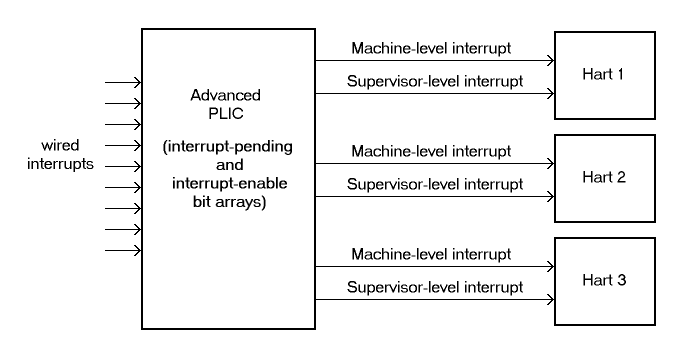
\includegraphics[scale=0.55]{figures/intrsWithoutIMSICs.png}}
    \caption{传统的有线中断发送方法,用于不支持 MSI 的 Hart}
    \label{fig:intrsWithoutIMSICs}
\end{figure}

如果没有 IMSIC,当前的高级中断架构不支持直接将外部中断信号发送到虚拟机,即使 {\RISCV} Hart 实现了特权架构的虚拟化扩展也是如此。相反,必须将中断发送到相关的虚拟机监管程序,然后该虚拟机监管程序可以选择向虚拟机注入虚拟中断。

\begin{commentary}
    如果 Hart 实现了虚拟化扩展,目前正在研究的一个问题是,是否应该允许 APLIC 将外部中断路由为虚拟化扩展的客户机外部中断,从而允许直接将中断发送到虚拟机,而无需在虚拟机监管程序级别处理每个中断。目前,我们假设需要直接向虚拟机发出外部中断信号的系统具有 IMSIC。
\end{commentary}

\begin{figure}[th]
    \centerline{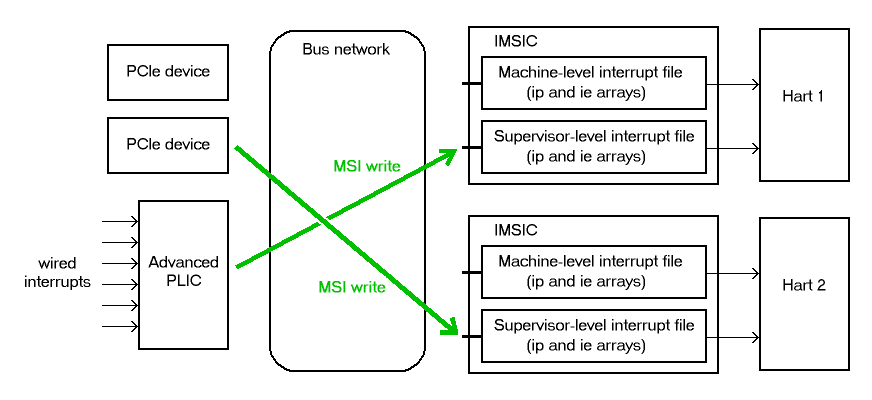
\includegraphics[scale=0.55]{figures/intrsWithIMSICs.png}}
    \caption{当 harts 具有 IMSIC 以接收 MSI 时,使用 MSI 进行中断发送。}
    \label{fig:intrsWithIMSICs}
\end{figure}

\subsubsection{有 IMSIC 的外部中断}

为了能够接收消息驱动中断,每个 {\RISCV} Hart 必须具有一个 IMSIC ,如图 \ref{fig:intrsWithIMSICs} 所示。基本上,消息驱动中断只是对硬件特定地址进行的内存写操作。为此,每个 IMSIC 在机器的地址空间中分配一个或多个不同的地址,当以预期的格式对其中一个地址进行写入时,对应的 IMSIC 将写入解释为相应 Hart 的外部中断。

由于所有 IMSIC 在机器的物理地址空间中具有唯一的地址,因此每个 IMSIC 可以从任何具有写入权限的代理 (Hart 或设备) 接收 MSI 写入。IMSIC 为针对 M 特权级和 S 特权级的 MSI 分别提供地址,一方面是为了通过控制不同地址的写入权限来单独授予或拒绝每个特权级上发送中断的能力,一方面是为了更好地支持虚拟化 (假设某特权级是更高特权级)。针对特定特权级的 MSI 被记录在 IMSIC 的中断文件 (interrupt file) 中,该文件主要由表示中断挂起位 (interrupt-pending bits) 的数组和表示该 Hart 当前准备接收哪个中断的中断使能位数组组成。

IMSIC 单元在第三章中完全定义。{\RISCV} 高级中断架构使用的 MSI 格式在该章节的第二节中进行了描述。

当 {\RISCV} 系统中的 Hart 具有 IMSIC 时,系统通常仍包含一个 APLIC,但其角色已改变。与图 \ref{fig:intrsWithoutIMSICs} 中直接通过线路向 Hart 发送中断信号不同,APLIC 将传入的有线中断转换为 MSI 写入,并通过它们的 IMSIC 单元将其发送到 Hart。每个 MSI 根据软件设置的 APLIC 配置被发送到单个目标 Hart。

如果 {\RISCV} Hart 实现了特权架构的虚拟化扩展,IMSICs 可能具有额外的客户机中断文件,用于向虚拟机传递中断。除了 IMSIC 的第三章,还可以查看专门介绍向虚拟机发送中断的第六章。如果系统还包含用于执行 I/O 设备内存访问的地址翻译的 IOMMU,则来自这些设备的 MSI 可能需要特殊处理。这个问题在第 8 章中得到了解决,即“用于向虚拟机传递 MSI 的 IOMMU 支持”。

\subsubsection{其他中断}

除了来自 I/O 设备的外部中断外,RISC-V 特权架构还指定了一些其他主要类别的中断用于 Hart。特权架构的时钟中断仍然得到充分支持,软件中断得到至少部分支持,尽管它们都没有出现在图 \ref{fig:intrsWithIMSICs} 和 \ref{fig:intrsWithoutIMSICs} 中。有关软件中断的具体信息,请参阅第七章“处理器间中断 (IPI, Inter-Processor Interrupts)”。

高级中断架构在 Hart 上添加了相当多的本地中断支持,即 Hart 在响应异步事件时本质上会自我中断,这些异步事件通常是错误。本地中断仍然包含在 Hart 内(或接近它),因此与标准的 RISC-V 时钟中断和软件中断一样,它们不会通过 APLIC 或 IMSIC。

\subsection{硬件中断标识}

{\RISCV} 特权架构为 Hart 的每个中断原因分配了一个独特的主要标识号 (major identity number),它是在中断陷入时自动写入 CSR \z{mcause} 或 \z{scause} 的异常代码。由特权架构标准化的中断原因的主要标识在 0-15 范围内,而编号 16 及以上则正式供平台标准或自定义使用。高级中断架构声称进一步控制范围在 16-23 和 32-47 的标识号,留下 24-31 范围内的编号和所有 48 及以上的主要标识号自定义使用。表 \ref{tab:interruptIdents} 描述了所有主要中断标识与此扩展的特征。

\begin{table*}[h!]
    \begin{center}
    \begin{tabular}{|c|c|l|}
    \hline
    Major identity & Minor identity & \\
    \hline
    \hline
    0              & --             & \em Reserved by Privileged Architecture \\
    \hline
    1              & --             & Supervisor software interrupt \\
    2              & --             & Virtual supervisor software interrupt \\
    3              & --             & Machine software interrupt \\
    \hline
    4              & --             & \em Reserved by Privileged Architecture \\
    \hline
    5              & --             & Supervisor timer interrupt \\
    6              & --             & Virtual supervisor timer interrupt \\
    7              & --             & Machine timer interrupt \\
    \hline
    8              & --             & \em Reserved by Privileged Architecture \\
    \hline
    9              & \multicolumn{1}{l|}{Determined by}
                                    & Supervisor external interrupt \\
    10             & \multicolumn{1}{l|}{\ external interrupt}
                                    & Virtual supervisor external interrupt \\
    11             & \multicolumn{1}{l|}{\ controller}
                                    & Machine external interrupt \\
    \hline
    12                   & -- & Supervisor guest external interrupt \\
    13                   & -- & Counter overflow interrupt \\
    14--15               & -- & \em Reserved by Privileged Architecture \\
    \hline
    \hline
    16--23         & --       & \em Reserved for standard local interrupts \\
    \hline
    24--31         & --       & \em Designated for custom use \\
    \hline
    32--34         & --       & \em Reserved for standard local interrupts \\
    35             & --       & Low-priority RAS event interrupt \\
    36--42         & --       & \em Reserved for standard local interrupts \\
    43             & --       & High-priority RAS event interrupt \\
    44--47         & --       & \em Reserved for standard local interrupts \\
    \hline
    $\geq \mbox{48}$ & --     & \em Designated for custom use \\
    \hline
    \end{tabular}
    \end{center}
    \caption{每个 hart 的所有中断原因的主要和次要标识。主要标识号 0-15 属于 {\RISCV} 特权架构的标准。}
    \label{tab:interruptIdents}
\end{table*}

大多数 I/O 设备的中断通过 Hart 的外部中断控制器传递到 Hart,它可以是 Hart 的 IMSIC(图 \ref{fig:intrsWithIMSICs})或 APLIC(图 \ref{fig:intrsWithoutIMSICs})。如表 \ref{tab:interruptIdents} 所示,给定特权级别的外部中断都共享一个单独的主要标识号:M 特权级为 11,S 特权级为 9,VS 特权级为 10。来自不同原因的外部中断通过外部中断控制器提供的次要标识号在 Hart 上互相区分。

除了外部中断之外,其他中断原因也可能有自己的次要标识号。然而,本文档只需要讨论外部中断的次要标识号。

高级中断架构定义的本地中断及其处理主要在第五章中讨论。

\subsection{选择接收中断的 Hart}

每个中断只会被传递给一个特权级别下的一个 Hart,通常由软件以某种方式确定。与其他某些架构不同,{\RISCV} 高级中断架构没有提供用于将中断广播或组播到多个 Hart 的标准硬件机制。

对于本地中断以及任何软件向 Hart 的较低特权级别注入的“虚拟”中断,这些中断完全是 Hart 本地的事务,其他 Hart 永远不可见。{\RISCV} 特权架构的时钟中断也与各自的 Hart 唯一绑定。

对于由 Hart 外部源接收的其他中断,软件会将每个中断信号(无论是通过线路还是通过 MSI 传递)配置为仅发送到单个 Hart。

要向多个 Hart 发送处理器间中断(IPI),发起 Hart 只需要执行一个循环,向每个目标 Hart 发送单个IPI即可。对于单个目标 Hart 的IPI,请参见第七章。

\begin{commentary}
    发送单个 IPI 到多个目的地时,源 Hart 所花费的工作量肯定会被接收 Hart 处理这些中断所花费的总工作量所压倒。因此,最好只期望提供自动化的 IPI 组播机制能在最好的情况下略微减少系统的总体工作量。对于非常大量的 Hart,IPI 组播的硬件机制必须解决软件如何在每次使用时指定预期目标集合的问题,而且实际的 IPI 物理传递与软件版本可能没有太大区别。

    我们不排除未来有可选的 IPI 组播硬件机制的可能性,但仅当在实际使用中可以证明具有显著优势时才会考虑。截至2020年,在拥有 IPI 组播硬件的系统上观察到 Linux 并没有使用该硬件机制。
\end{commentary}

在极少数情况下,需要将来自 I/O 设备的单个中断发送给多个 Hart,这个中断必须发送到一个单独的 Hart,然后该 Hart 可以通过IPI向其他 Hart 发出中断。

\begin{commentary}
我们认为,I/O 中断通知多个 Hart 的情况非常罕见,因此在这种情况下不能证明标准化硬件支持组播的必要性。
\end{commentary}

\begin{commentary}
除了组播传递之外,其他架构还支持“1-of-$N$”中断传递选项,其中硬件从配置的 $N$ 个 Hart 中选择一个单一的目标 Hart,旨在在 Hart 之间自动平衡中断处理的负载。2010年代的实验对 1-of-$N$ 模式的效用提出了质疑,在实践中显示出软件通常可以比实际芯片中实现的硬件算法更好地平衡负载。因此,Linux 被修改为停止在拥有 1-of-$N$ 中断传递的系统上使用该功能。

我们仍然认为,硬件负载平衡中断处理可能对某些专业市场(如网络)有益,但是迄今为止在这方面所做的声明不能证明要求所有 {\RISCV} 服务器支持 1-of-$N$ 传递。有了更多的证据,某些 1-of-$N$ 传递机制可能成为未来的选择。
\end{commentary}

\begin{commentary}
    最初的 {\RISCV} 平台级中断控制器(PLIC)是可配置的,因此每个中断源可以向任何 Hart 子集(可能是所有 Hart)发出外部中断信号。当多个 Hart 从 PLIC 收到单个原因的外部中断时,首先在PLIC上“声明”中断的 Hart 将负责对其进行服务。通常,这会产生竞争,其中配置为接收多播中断的 Hart 子集同时接收外部中断并竞争成为在 PLIC 上首先声明中断的 Hart。意图是提供一种 1-of-$N$ 中断传递形式。但是,对于所有未能获得声明的 Hart,其中断陷入的开销都会被浪费。
    
    出于已经给出的原因,APLIC 支持将每个中断仅发送到由软件选择的单个 Hart,而不是多个 Hart。
\end{commentary}

\subsection{ISA 扩展 Smaia 和 Ssaia}

高级中断架构(AIA)为 {\RISCV} 指令集架构(ISA)的扩展定义了两个名称,一个用于 M 特权级,另一个用于 S 特权级。对于 M 特权级,扩展名 \textbf{Smaia} 涵盖了AIA为 Hart 指定的所有特权级别上所有添加的 CSR 和所有修改的中断响应行为。对于 S 特权级,扩展名 \textbf{Ssaia} 与 Smaia 基本相同,但排除了 M 特权级的 CSR 和 S 特权级看不到的行为。

扩展名 Smaia 和 Ssaia 仅涵盖对 Hart 的 ISA 产生影响的那些 AIA 特性。虽然下文将 APLIC、IOMMU 和除写入 IMSIC 之外的任何启动处理器间中断的机制描述或讨论为 AIA 的一部分,但它们不被 Smaia 或Ssaia提及,因为这些组件被归类为非 ISA 的组件。

正如后续章节所展示的,AIA 具体添加的 CSR 和行为,即 Smaia 或 Ssaia 所提及的,取决于基础 ISA 的 XLEN(RV32 或 RV64),是否实现了 S-mode 和虚拟化扩展,以及 Hart 是否具有IMSIC。但并没有为每个可能的有效子集提供单独的 AIA 扩展名。相反,不同的组合可以从指示的特性(例如RV64I+S-mode+Smaia,但不包括虚拟化扩展)的交集中推断出来。

像编译器和汇编器这样的软件开发工具不需要关心 IMSIC 是否存在,而是应该只允许尝试访问 IMSIC CSR(在第二章和第三章中描述),如果指示了 Smaia 或 Ssaia。如果没有实际的 IMSIC,这样的尝试可能会触发异常并陷入,但对于开发工具来说,这不是一个问题。

\section{Hart 中添加的控制状态寄存器(CSR)}

对于{\RISCV} Hart 可以接收中断并陷入的每个特权级别,高级中断架构都添加了用于中断控制和处理的 CSR。

\subsection{M 特权级 CSR}

表 \ref{tab:CSRs-M} 列出了在 M 特权级添加的 CSR 以及大小被高级中断架构更改的现有的 M 特权级 CSR。现有的CSR \z{mie}、\z{mip}和\z{mideleg}被扩展为64位以支持总共64个中断原因。

\begin{table*}[h!]
    \begin{center}
    \begin{tabular}{|c|c|c|l|l|}
    \hline
    Number & Privilege & Width & Name & Description \\
    \hline
    \hline
    \multicolumn{5}{|c|}{Machine-Level Window to Indirectly Accessed Registers} \\
    \hline
    \z{0x350} & MRW & XLEN  & \z{miselect} & Machine indirect register select \\
    \z{0x351} & MRW & XLEN  & \z{mireg}    & Machine indirect register alias \\
    \hline
    \multicolumn{5}{|c|}{Machine-Level Interrupts} \\
    \hline
    \z{0x304} & MRW & 64    & \z{mie}    & Machine interrupt-enable bits \\
    \z{0x344} & MRW & 64    & \z{mip}    & Machine interrupt-pending bits \\
    \z{0x35C} & MRW & MXLEN & \z{mtopei}
                                  & Machine top external interrupt (only with an \\
              &     &       &            & \quad IMSIC) \\
    \z{0xFB0} & MRO & MXLEN & \z{mtopi}  & Machine top interrupt \\
    \hline
    \multicolumn{5}{|c|}{Delegated and Virtual Interrupts for Supervisor Level} \\
    \hline
    \z{0x303} & MRW & 64 & \z{mideleg} & Machine interrupt delegation \\
    \z{0x308} & MRW & 64 & \z{mvien}   & Machine virtual interrupt enables \\
    \z{0x309} & MRW & 64 & \z{mvip}    & Machine virtual interrupt-pending bits \\
    \hline
    \multicolumn{5}{|c|}{Machine-Level High-Half CSRs (RV32 only)} \\
    \hline
    \z{0x313} & MRW & 32 & \z{midelegh}
                            & Upper 32 bits of of \z{mideleg} (only with S-mode) \\
    \z{0x314} & MRW & 32 & \z{mieh} & Upper 32 bits of \z{mie} \\
    \z{0x318} & MRW & 32 & \z{mvienh}
                                 & Upper 32 bits of \z{mvien} (only with S-mode) \\
    \z{0x319} & MRW & 32 & \z{mviph}
                                  & Upper 32 bits of \z{mvip} (only with S-mode) \\
    \z{0x354} & MRW & 32 & \z{miph} & Upper 32 bits of \z{mip} \\
    \hline
    \end{tabular}
    \end{center}
    \caption{高级中断体系结构添加或扩展的 M 特权级 CSR}
    \label{tab:CSRs-M}
\end{table*}

对于RV32,表中列出的高半部 CSR 允许访问寄存器 \z{mideleg}、\z{mie}、\z{mvien}、\z{mvip} 和 \z{mip} 的高32位。高级中断架构要求这些高半部 CSR 存在于RV32中,但它们访问的位可能都是只读的零。

CSR \z{miselect} 和 \z{mireg} 提供了访问表 \ref{tab:CSRs-M}中以外的多个寄存器的窗口。\z{miselect} 的值确定当前可以通过别名 CSR \z{mireg}访问哪个寄存器。\z{miselect} 是一个 {\WARL} 寄存器,它必须支持一定范围的最小值,这取决于实现的特性。当没有实现 IMSIC 时,\z{miselect}必须能够至少容纳 0 到 \z{0x3F} 范围内的任何6位值。当实现了 IMSIC 时,\z{miselect} 必须能够容纳 0 到 \z{0xFF} 范围内的任何8位值。目前,范围在 0 到 \z{0xFF} 之间的 \z{miselect} 值被分配为以下子范围:

\begin{displayLinesTable}[l@{\quad}l]
    \z{0x00}--\z{0x2F} & reserved \\
    \z{0x30}--\z{0x3F} & major interrupt priorities \\
    \z{0x40}--\z{0x6F} & reserved \\
    \z{0x70}--\z{0xFF} & external interrupts (only with an IMSIC) \\
\end{displayLinesTable}
\z{miselect}也可能支持范围在 \z{0x00}--\z{0xFF} 之外的值,尽管目前没有标准寄存器分配给超过 \z{0xFF} 的值。

具有最高有效位($\mbox{XLEN-1}=\mbox{1}$)的 \z{miselect} 值指定为自定义使用,可能是用于通过 \z{mireg} 访问自定义寄存器。如果 XLEN 更改,则 \z{miselect} 的最高有效位移动到新位置,保留其之前的值。实现不需要支持 \z{miselect} 的任何自定义值。

当 \z{miselect} 是保留范围内的数字(当前为 \z{0x00}--\z{0x2F},\z{0x40}--\z{0x6F},或未指定为自定义使用的数字以上\z{0xFF}),尝试访问\z{mireg}通常会引发非法指令异常。

通常,仅当实现了IMSIC时,外部中断的范围 \z{0x70}--\z{0xFF} 才会被填充。否则,在 \z{miselect} 处于此范围时尝试访问 \z{mireg} 也会导致非法指令异常。外部中断区域的内容在 IMSIC 章节(第三章)中有所说明。

当实现了IMSIC时,CSR \z{mtopei} 也只存在于 IMSIC 间接访问的寄存器中,因此在 IMSIC 章节(第 三 章)中有所说明。

CSR \z{mtopi} 报告了挂起并启用的优先级最高的机器级中断,如第五章所述。

当实现 \mbox{S-mode} 时,CSR \z{mvien}和\z{mvip}支持监管模式的中断过滤和虚拟中断。这些功能在第五章第三节中解释。

\subsection{S 特权级 CSR}

如果 Hart 实现 \mbox{S-mode},表 \ref{tab:CSRs-S} 列出了在 S 特权级添加的 CSR 以及大小被高级中断架构更改的现有的 S 特权级 CSR。这些寄存器的功能都与 M 特权级对应。

\begin{table*}[h!]
    \begin{center}
    \begin{tabular}{|c|c|c|l|l|}
    \hline
    Number & Privilege & Width & Name      & Description \\
    \hline
    \hline
    \multicolumn{5}{|c|}{%
      Supervisor-Level Window to Indirectly Accessed Registers} \\
    \hline
    \z{0x150} & SRW & XLEN  & \z{siselect} & Supervisor indirect register select \\
    \z{0x151} & SRW & XLEN  & \z{sireg}    & Supervisor indirect register alias \\
    \hline
    \multicolumn{5}{|c|}{Supervisor-Level Interrupts} \\
    \hline
    \z{0x104} & SRW & 64    & \z{sie}      & Supervisor interrupt-enable bits \\
    \z{0x144} & SRW & 64    & \z{sip}      & Supervisor interrupt-pending bits \\
    \z{0x15C} & SRW & SXLEN & \z{stopei}
                                       & Supervisor top external interrupt (only \\
              &     &       &          & \quad with an IMSIC) \\
    \z{0xDB0} & SRO & SXLEN & \z{stopi}    & Supervisor top interrupt \\
    \hline
    \multicolumn{5}{|c|}{Supervisor-Level High-Half CSRs (RV32 only)} \\
    \hline
    \z{0x114} & SRW & 32    & \z{sieh}     & Upper 32 bits of \z{sie} \\
    \z{0x154} & SRW & 32    & \z{siph}     & Upper 32 bits of \z{sip} \\
    \hline
    \end{tabular}
    \end{center}
    \caption{高级中断体系结构添加或扩展的 S 特权级 CSR}
    \label{tab:CSRs-S}
\end{table*}

可通过 \z{siselect}/\z{sireg} 窗口访问的寄存器空间与 M 特权级的寄存器空间是独立的,但是与之平行,用于 S 特权级中断而不是 M 特权级中断。范围在 0 到 \z{0xFF} 内的 \z{siselect} 分配的值如下

\begin{displayLinesTable}[l@{\quad}l]
    \z{0x00}--\z{0x2F} & reserved \\
    \z{0x30}--\z{0x3F} & major interrupt priorities \\
    \z{0x40}--\z{0x6F} & reserved \\
    \z{0x70}--\z{0xFF} & external interrupts (only with an IMSIC) \\
\end{displayLinesTable}

为了最大限度地提高兼容性,建议 \z{siselect} 至少支持 9 位的范围,即 0 到 \z{0x1FF},无论是否存在IMSIC。

\begin{commentary}
由于 VS CSR \z{vsiselect}(第二章第三节)始终具有至少 9 位,而且像其他 VS CSR 一样,在虚拟机(\mbox{VS-mode}或\mbox{VU-mode})中执行时,\z{vsiselect} 代替 \z{siselect},实现较小的 \z{siselect} 范围允许软件发现它没有在虚拟机中运行。
\end{commentary}

与 \z{miselect} 一样,具有最高有效位($\mbox{XLEN-1}=\mbox{1}$)的 \z{siselect} 值指定为自定义使用。如果 XLEN 更改,则 \z{siselect} 的最高有效位移动到新位置,保留其之前的值。实现不需要支持\z{siselect} 的任何自定义值。

当 \z{siselect} 是保留范围内的数字(当前为 \z{0x00}--\z{0x2F},\z{0x40}--\z{0x6F},或未指定为自定义使用的数字以上 \z{0xFF}),或在没有IMSIC的情况下处于 \z{0x70}--\z{0xFF}范围内时,尝试访问 \z{sireg} 应尽可能引发非法指令异常(除非在虚拟机中执行,下一节讨论)。

请注意,\z{siselect} 和 \z{sireg} 的宽度始终为当前的 XLEN,而不是 SXLEN。因此,例如,如果 MXLEN = 64 且 SXLEN = 32,则当当前特权模式为 M(运行RV64代码)时,这些寄存器为 64 位,但特权模式为 S(RV32代码)时为32位。

CSR \z{stopei} 在IMSIC章节(第三章)中有所描述。

寄存器 \z{stopi} 报告了挂起并启用的优先级最高的监管级别中断,如第五章所述。

\subsection{Hypervisor 和 VS 特权级 CSR}

如果 Hart 实现了特权架构的虚拟化扩展,则表 \ref{tab:CSRs-hypervisor} 中列出的虚拟化管理程序(Hypervisor)和 VS CSR 也将被添加或扩展为 64 位。

\begin{table*}[h!]
    \begin{center}
    \begin{tabular}{|c|c|c|l|l|}
    \hline
    Number & Privilege & Width & Name & Description \\
    \hline
    \hline
    \multicolumn{5}{|c|}{%
      Delegated and Virtual Interrupts, Interrupt Priorities, for VS Level%
    } \\
    \hline
    \z{0x603} & HRW & 64     & \z{hideleg} & Hypervisor interrupt delegation \\
    \z{0x608} & HRW & 64     & \z{hvien}  & Hypervisor virtual interrupt enables \\
    \z{0x609} & HRW & HSXLEN & \z{hvictl} & Hypervisor virtual interrupt control \\
    \z{0x645} & HRW & 64     & \z{hvip}
                                     & Hypervisor virtual interrupt-pending bits \\
    \z{0x646} & HRW & 64     & \z{hviprio1}
                                     & Hypervisor VS-level interrupt priorities \\
    \z{0x647} & HRW & 64     & \z{hviprio2}
                                     & Hypervisor VS-level interrupt priorities \\
    \hline
    \multicolumn{5}{|c|}{VS-Level Window to Indirectly Accessed Registers} \\
    \hline
    \z{0x250} & HRW & XLEN   & \z{vsiselect}
                                   & Virtual supervisor indirect register select \\
    \z{0x251} & HRW & XLEN   & \z{vsireg}
                                   & Virtual supervisor indirect register alias \\
    \hline
    \multicolumn{5}{|c|}{VS-Level Interrupts} \\
    \hline
    \z{0x204} & HRW & 64     & \z{vsie}
                                     & Virtual supervisor interrupt-enable bits \\
    \z{0x244} & HRW & 64     & \z{vsip}
                                     & Virtual supervisor interrupt-pending bits \\
    \z{0x25C} & HRW & VSXLEN & \z{vstopei}
                               & Virtual supervisor top external interrupt (only \\
              &     &        & & \quad with an IMSIC) \\
    \z{0xEB0} & HRO & VSXLEN & \z{vstopi} & Virtual supervisor top interrupt \\
    \hline
    \multicolumn{5}{|c|}{Hypervisor and VS-Level High-Half CSRs (RV32 only)} \\
    \hline
    \z{0x613} & HRW & 32     & \z{hidelegh}  & Upper 32 bits of \z{hideleg} \\
    \z{0x618} & HRW & 32     & \z{hvienh}    & Upper 32 bits of \z{hvien} \\
    \z{0x655} & HRW & 32     & \z{hviph}     & Upper 32 bits of \z{hvip} \\
    \z{0x656} & HRW & 32     & \z{hviprio1h} & Upper 32 bits of \z{hviprio1} \\
    \z{0x657} & HRW & 32     & \z{hviprio2h} & Upper 32 bits of \z{hviprio2} \\
    \z{0x214} & HRW & 32     & \z{vsieh}     & Upper 32 bits of \z{vsie} \\
    \z{0x254} & HRW & 32     & \z{vsiph}     & Upper 32 bits of \z{vsip} \\
    \hline
    \end{tabular}
    \end{center}
    \caption{高级中断体系结构添加或扩展的 Hypervisor 和 VS 特权级 CSR 。参数 HSXLEN 只是扩展的 S 模式的 SXLEN 的另一个名称。}
    \label{tab:CSRs-hypervisor}
\end{table*}

表中的新 VS CSR(\z{vsiselect},\z{vsireg},\z{vstopei} 和 \z{vstopi})都与S 特权级 CSR匹配,并在虚拟机(在\mbox{VS-mode}或\mbox{VU-mode}中)执行时替换这些 S 特权级 CSR。

CSR \z{vsiselect} 需要支持至少 0 到 \z{0x1FF} 范围的 9 位,无论是否实现IMSIC。与 \z{siselect} 类似,\z{vsiselect} 的具有最高有效位($\mbox{XLEN-1}=\mbox{1}$)的值指定为自定义使用。如果XLEN 更改,则 \z{vsiselect} 的最高有效位移动到新位置,保留其之前的值。

与 \z{siselect} 和 \z{sireg} 一样,\z{vsiselect} 和 \z{vsireg} 的宽度始终为当前的 XLEN ,而不是 VSXLEN。因此,例如,如果 HSXLEN = 64 且 VSXLEN = 32,则当在 HS 模式下运行 RV64 代码的虚拟化管理程序访问这些寄存器时,它们为 64 位,但在在 VS 模式下运行 RV32 代码的客户操作系统访问这些寄存器时为32位。

\z{vsiselect} 可选择的寄存器空间比 M 特权级和 S 特权级更有限:

\begin{displayLinesTable}[l@{\quad}l]
    \z{0x000}--\z{0x02F} & reserved \\
    \z{0x030}--\z{0x03F} & inaccessible \\
    \z{0x040}--\z{0x06F} & reserved \\
    \z{0x070}--\z{0x0FF} & external interrupts (IMSIC only), or inaccessible \\
    \z{0x100}--\z{0x1FF} & reserved \\
\end{displayLinesTable}

当 \z{vsiselect} 具有不可访问寄存器的编号时,尝试从 M 模式或 HS 模式访问 \z{vsireg} 会引发非法指令异常,而尝试从 VS 模式或 VU 模式访问 \z{sireg}(实际上是 \z{vsireg})会引发虚拟指令异常。类似地,当 \z{vsiselect} 具有保留值时,包括未设置最高有效位的 \z{0x1FF} 以上的值,从 M 模式或 HS 模式访问 \z{vsireg} 应最好引发非法指令异常,而尝试从 VS 模式或 VU 模式访问 \z{sireg}(实际上是 \z{vsireg})应最好引发虚拟指令异常。

\begin{commentary}
要求 \z{vsiselect} 的范围为 {\rm 0}--\z{0x1FF},即使大部分或全部空间都被保留或不可访问,也允许虚拟化管理程序模拟已实现范围内间接访问的寄存器,包括可能在未来标准化 \z{0x100}--\z{0x1FF} 的寄存器。
\end{commentary}

外部中断寄存器的位置(编号为 \z{0x70}--\z{0xFF})仅在 \z{hstatus} 的 VGEIN 字段是已实现的客户机外部中断号,而不是 0 时才可访问。如果VGEIN不是已实现的客户机外部中断号(包括未实现IMSIC的情况),则所有非自定义值的 \z{vsiselect} 要么保留,要么指定不可访问的寄存器。

同样地,当 \z{hstatus}.VGEIN 不是已实现的客户机外部中断号时,尝试从 M 模式或 HS 模式访问 CSR \z{vstopei} 会引发非法指令异常,而尝试从 VS 模式访问 \z{stopei} 会引发虚拟指令异常。

表 \ref{tab:CSRs-hypervisor} 中的新虚拟化管理程序 CSR(\z{hvien},\z{hvictl},\z{hviprio1}和\z{hviprio2})增强了向 VS 级别注入中断的 \z{hvip}。这些寄存器的使用在第六章虚拟机中断有所涉及。

\subsection{虚拟指令异常}

遵循虚拟机扩展的默认规则,从 VS 模式尝试直接访问虚拟化管理程序或 VS CSR,或从 VU 模式访问任何 S 特权级的 CSR(包括虚拟化管理程序和 VS CSR),通常不会引发非法指令异常,而是引发虚拟指令异常。有关详细信息,请参阅 {\RISCV} 特权架构。

\subsection{通过状态使能寄存器的访问控制}

如果扩展 Smstateen 与高级中断架构(AIA)一起实现,那么状态使能寄存器 \z{mstateen0} 的三个位将控制特权模式低于 M 模式的状态访问 AIA 添加的状态。

\begin{displayLinesTable}[l@{\quad}l]
    bit 60 & CSRs \z{siselect}, \z{sireg}, \z{vsiselect}, and \z{vsireg} \\
    bit 59 & all other state added by the AIA
              and not controlled by bits 60 and 58 \\
    bit 58 & all IMSIC state, including CSRs \z{stopei} and \z{vstopei} \\
\end{displayLinesTable}

如果 \z{mstateen0} 中的其中一个位为零,则尝试从低于 M 模式的特权模式访问相应的状态将导致非法指令异常。与往常一样,状态使能 CSR 不影响在 M 模式下的任何状态的可访问性,只在低于 M 模式的特权模式下生效。有关更多说明,请参阅 ISA 扩展 Smstateen 的文档。

位 59 控制对 AIA CSR \z{siph}、\z{sieh}、\z{stopi}、\z{hidelegh}、\z{hvien}/\z{hvienh}、\z{hviph}、\z{hvictl}、\z{hviprio1}/\z{hviprio1h}、\z{hviprio2}/\z{hviprio2h}、\z{vsiph}、\z{vsieh} 和 \z{vstopi} 的访问,以及通过 \z{siselect} + \z{sireg} 访问的监管级中断优先级(第五章的 \z{iprio} 数组)。

位 58 仅在 Hart 有 IMSIC 时在 \z{mstateen0} 中实现。如果 Hypervisor 扩展也被实现,则该位不影响 Hypervisor CSR \z{hgeip} 和 \z{hgeie} 或 \z{hstatus} 的 VGEIN 字段的行为或可访问性。特别是,即使 \z{mstateen0} 的位 58 为零,IMSIC 中的客户机外部中断仍将在 \mbox{HS-mode} 中的 \z{hgeip} 中可见。

\begin{commentary}
Smstateen 的早期一个未经批准的草案指出,当 \z{mstateen0} 的位 58 为 0 时,\z{hgeip}、\z{hgeie} 和 \z{hstatus} 的 VGEIN 字段都是只读的 0 。这种影响不再正确。
\end{commentary}

如果 Hypervisor 扩展被实现,那么相同的三个位也在 Hypservisor CSR \z{hstateen0} 中定义,但只涉及在特权模式 VS 和 VU 中执行的虚拟机可能可访问的状态:

\begin{displayLinesTable}[l@{\quad}l]
    bit 60 & CSRs \z{siselect} and \z{sireg}
              (really \z{vsiselect} and \z{vsireg}) \\
    bit 59 & CSRs \z{siph} and \z{sieh} (RV32 only) and \z{stopi} \\
           &   (really \z{vsiph}, \z{vsieh}, and \z{vstopi}) \\
    bit 58 & all state of IMSIC guest interrupt files, \\
           &   including CSR \z{stopei} (really \z{vstopei}) \\
\end{displayLinesTable}

如果 \z{hstateen0} 中的一个位为零,并且相应的位在 \z{mstateen0} 中为一,则尝试从 VS 或 \mbox{VU-mode} 访问相应的状态将引发虚拟指令异常。(但请注意,对于高半部 CSR \z{siph} 和 \z{sieh},仅当 XLEN = 32 时才适用。当 $\mbox{XLEN} > \mbox{32}$ 时,访问 \z{siph} 或 \z{sieh} 将像通常一样引发非法指令异常,而不是虚拟指令异常。)

位 58 仅在 hart 有 IMSIC 时在 \z{hstateen0} 中实现。此外,即使有 IMSIC,如果 IMSIC 没有用于客户机外部中断的客户机中断文件(第三章),位 58 也可能(或可能不)在 \z{hstateen0} 中为只读零。当此位为零时(无论是只读零还是设为零),虚拟机将无法访问 Hart 的 IMSIC,就像 \z{hstatus}.VGEIN = 0 一样。

扩展 Ssstateen 被定义为 Smstateen 的 S 特权级视图。因此,Ssaia 和 Ssstateen 的组合包含了上面为 \z{hstateen0} 定义的位,但不包括 \z{mstateen0} 的位,因为 M 特权级 CSRs 对 S 特权级不可见。

\section{IMSIC}

传入 MSI 控制器(IMSIC)是一个可选的 {\RISCV} 硬件组件,与一个 Hart 紧密耦合,每个 Hart 有一个 IMSIC。IMSIC 接收和记录 Hart 收到的消息驱动中断(MSI),并在有待处理的已启用中断时向 Hart 发送中断信号。

IMSIC 在机器的地址空间中有一个或多个内存映射寄存器用于接收 MSI。除了这些内存映射寄存器之外,软件主要通过连接 IMSIC 的 Hart 上几个 {\RISCV} CSR 与 IMSIC 进行交互。

\subsection{中断文件和中断标识}

在{\RISCV}系统中,MSI不仅可以定向到特定的 Hart,还可以定向到特定 Hart 的特定特权级,例如 M 特权级或 S 特权级。此外,当 Hart 实现虚拟化扩展时,IMSIC可以选择允许 MSI 定向到 VS 特权级的特定虚拟 Hart。

对于可以将 MSI 定向到 Hart 的每个特权级和每个虚拟 Hart,Hart 对应的 IMSIC 都包含一个单独的中断文件。假设 Hart 实现了 S 模式,它的 IMSIC 至少有两个中断文件,一个用于 M 特权级,另一个用于 S 特权级。当 Hart 还实现了虚拟化扩展时,它的 IMSIC 可能会有额外的中断文件用于虚拟 Hart,称为客户机中断文件。IMSIC 为虚拟Hart 提供的客户机中断文件的数量正好是 GEILEN ,即由 {\RISCV} 特权架构定义的虚拟化扩展支持的客户机外部中断数量。

每个单独的中断文件主要由两个相同大小的位数组组成,一个数组用于记录到达但尚未服务的 MSI(中断挂起位),另一个数组用于指定 Hart 当前可接受哪些中断(中断使能位)。每个位在两个数组中对应着一个不同的中断标识号,用于区分来自不同源的 MSI。由于 IMSIC 是附加到 Hart 的外部中断控制器,因此中断文件的中断标识成为连接的 Hart 的外部中断的次要标识。

中断文件支持的中断标识数(即每个数组中的活动位数)比 64 的倍数少一个,最少为 63,最多为2047。

\begin{commentary}
    平台标准可以增加每个中断文件必须实现的最小中断标识数。
\end{commentary}

当一个中断文件支持 $N$ 个不同的中断标识时,有效的标识号在 1 到 $N$ 之间(包括 1 和 $N$)。在这个范围内的标识号被认为是中断文件实现的;范围外的号码则没有被实现。数字0永远不是一个有效的中断标识。

IMSIC 硬件不会假设一个中断文件中的中断标识号与另一个中断文件中的中断标识号之间存在任何连接。通常期望软件将相同的中断标识号分配给不同的中断文件中不同的 MSI 源,而无需跨中断文件进行协调。因此,在系统中可以单独区分的 MSI 源的总数可能是单个中断文件中中断标识数乘以系统中所有 Hart 上中断文件的总数的乘积。

并非所有系统中的中断文件都具有相同的大小(实现相同数量的中断标识)。对于给定的 Hart,客户机外部中断的中断文件必须具有相同的大小,但是 M 特权级和 S 特权级的中断文件的大小可能与客户机外部中断的中断文件的大小不同且互不相同。同样,不同 Hart 的中断文件大小可能不同。

平台可能提供一种方式让软件配置 IMSIC 中中断文件的数量和/或大小,例如允许在 M 特权级上使用较小的中断文件来交换更大的 S 特权级的中断文件,反之亦然。
任何这样的可配置性都不在本规范的讨论范围之内,但是建议只有 M 特权级才能控制 IMSIC 中中断文件的数量和大小。

\subsection{MSI 编码}

已经建立的标准(特别是 PCI 和 PCI Express)规定,设备发出的每个单独的消息驱动中断(MSI)都采用设备进行自然对齐的32位写入形式,地址和值都由软件在设备(或设备控制器)上进行配置。根据设备或控制器符合的标准版本,地址可能被限制在较低的 4-GiB(32位)范围内,并且写入的值可能限制在 16 位范围内,其中高 16 位始终为零。

当 {\RISCV} Hart 具备 IMSIC 时,设备发出的 MSI 通常直接发送到由软件选择处理中断的特定 Hart(可能基于某种中断亲和策略)。MSI 通过存在于接收 Hart 的IMSIC中的相应中断文件来定向到特定特权级或虚拟 Hart。MSI 写入地址是连接到目标中断文件的特定字长寄存器的物理地址。MSI 写入数据只是要在该中断文件中挂起的中断的标识号(最终成为对应 Hart 的外部中断的次要标识)。

通过在设备上配置 MSI 的地址和数据,系统软件完全控制:
(a)哪个 Hart 接收特定设备中断,
(b)目标特权级别或虚拟 Hart,
(c)代表目标中断文件中 MSI 的标识号。
其中 a 和 b 由 MSI 写入地址对应的中断文件确定,而 c 由 MSI 写入数据确定。

\begin{commentary}
由于 IMSIC 支持的最大中断标识号为 2047,因此对 MSI 数据的 16 位限制没有问题。
\end{commentary}

当实现了虚拟化扩展并且设备直接由客户操作系统管理时,设备发出的 MSI 地址最初是客户机物理地址,因为它们是由客户机操作系统在设备上配置的。这些客户机地址必须由 IOMMU 进行翻译,由虚拟机监控程序配置 IOMMU 来将这些 MSI 重定向到正确的客户机外部中断的中断文件中。有关此主题的更多信息,请参见第八章。

\subsection{中断优先级}

在单个中断文件中,中断优先级直接由中断标识号确定。较低的标识号具有较高的优先级。

\begin{commentary}
    由于 MSI 让软件完全控制中断文件中标识号的分配,因此软件可以自由选择反映所需中断相对优先级的标识号。

    确实,如果中断文件包括要分配给每个中断标识的优先级数字的数组,软件可以更动态地调整中断优先级。然而,我们认为这种额外的灵活性不会经常被利用,以至于不能证明其所需的额外硬件开销。实际上,对于许多当前使用 MSI 的系统,软件通常会完全忽略中断优先级,并表现得好像所有中断具有相同的优先级。
\end{commentary}

\begin{commentary}
    中断文件的最低标识号被赋予了最高的优先级,而不是反向顺序,因为仅对于最高优先级的中断,优先级顺序可能需要仔细管理,而保证在所有系统中存在的是较低的编号 1 到63(或者可能是 1 到 255)。例如,考虑中断文件的最高优先级中断,最紧急的中断总是标识号1。如果优先顺序被反转,最高优先级的中断将在不同的机器上具有不同的标识号,具体取决于中断文件实现了多少个标识号。软件能够为最高优先级的中断分配固定的标识号,这被认为是值得的,即使中断优先级与自然数字顺序相反可能有些奇怪。
\end{commentary}

\subsection{复位和状态}

当 IMSIC 复位时,其所有中断文件的状态都变得有效和一致,但除此之外的状态是未指定的,可能会有例外情况,例如 M 特权级和 S 特权级中断文件的 \z{eidelivery} 寄存器,详见第八节。

如果 IMSIC 包含 S 特权级中断文件,并且连接的硬件上的软件启用了之前被禁用的 \mbox{S-mode}(例如通过将CSR \z{misa} 的位 S 从 0 更改为1),则 S 特权级中断文件的所有状态都是有效和一致的,但除此之外的状态是未指定的。

同样地,如果 IMSIC 包含客户机中断文件,并且连接的硬件上的软件启用了之前被禁用的虚拟化扩展(例如通过将 \z{misa} 的位 H 从 0 更改为 1),则 IMSIC 的客户机中断文件的所有状态都是有效和一致的,但除此之外的状态是未指定的。

\subsection{中断文件的地址范围}

IMSIC中的每个中断文件都有一个或两个内存映射的 \mbox{32 位} 寄存器,用于接收 MSI 写入。这些内存映射的寄存器位于一个自然对齐的 \mbox{4-KiB} 物理地址空间区域内(一页),即每个中断文件一个页面。

中断文件的地址范围布局如下:

\begin{displayLinesTable}[l@{\quad}l@{\qquad}l]
    offset    & \ size  & register name \\
    \noalign{\medskip}
    \z{0x000} & 4 bytes & \z{seteipnum\_le} \\
    \z{0x004} & 4 bytes & \z{seteipnum\_be} \\
\end{displayLinesTable}

中断文件的 4-KiB 地址范围中的所有其他字节都是保留的,并且必须实现为只读零。在中断文件的地址范围内,仅支持自然对齐的 \mbox{32 位} 简单读写。写入只读字节会被忽略。对于其他形式的访问(其他大小、不对齐的访问或 AMO),IMSIC 实现应该优先报告访问故障或总线错误,否则必须忽略该访问。

如果 $i$ 是一个实现的中断标识号,将值 $i$ 以小端字节顺序写入 \z{seteipnum\_le}(按编号设置外部中断挂起位,小端字节顺序),会导致中断 $i$ 的挂起位被设置为1。如果写入的值不是以小端字节顺序表示的实现的中断标识号,则会忽略对 \z{seteipnum\_le} 的写入。

对于支持大端字节顺序的系统,如果 $i$ 是实现的中断标识号,则将值 $i$ 以大端字节顺序写入 \z{seteipnum\_be}(按编号设置外部中断挂起位,大端字节顺序)会导致中断 $i$ 的挂起位被设置为1。如果写入的值不是以大端字节顺序表示的实现的中断标识号,则会忽略对 \z{seteipnum\_be} 的写入。仅支持小端字节顺序的系统可以选择忽略对 \z{seteipnum\_be} 的所有写入。

在大多数系统中,\z{seteipnum\_le} 是用于定向到该中断文件的 MSI 的写入端口。对于主要为大端字节顺序构建的系统,\z{seteipnum\_be} 可能为某些设备定向到该中断文件的 MSI 的写入端口。

无论何种情况,对 \z{seteipnum\_le} 或 \z{seteipnum\_be} 的读取都返回零。

当不被忽略时,对中断文件的地址范围的写入保证最终反映在中断文件中,但不一定是立即的。对于单个中断文件,对其地址范围的多个写入(存储),虽然具有任意的延迟,但总是按照 {\RISCV} 非特权指令集所定义的存储指令的全局内存顺序 (global memory order) 发生。

\begin{commentary}
    在大多数情况下,对中断文件地址范围的写入完成后,写入对中断文件的影响的任何延迟都与内存系统中的其他延迟无法区分。然而,如果一个Hart向自己的IMSIC的 \z{seteipnum\_le} 或 \z{seteipnum\_be} 寄存器写入数据,则存储指令完成和中断文件中相应的中断挂起位设置之间的延迟可能对 Hart 可见。
\end{commentary}

\subsection{多个中断文件的地址布局}

IMSIC 实现的每个中断文件都有自己的内存区域,如前一节所述,占用机器地址空间的一个 \mbox{4-KiB} 页面。在实践中,所有 IMSIC 的 M 特权级中断文件的内存页应该位于地址空间的一个部分中,并且所有 S 特权级和客户机中断文件的内存页应该类似地位于地址空间的另一个部分中,按照以下规则。

\begin{commentary}
    将 M 特权级中断文件与地址空间中的其他中断文件分开的主要原因是,实现物理内存保护(PMP)的 Hart 可以仅使用一个 PMP 表项授予 S 特权级访问所有 S 特权级和客户机中断文件。如果 M 特权级中断文件的内存页面与低特权级的中断文件相间排列,那么在授予 S 特权级访问所有非机器级中断文件时所需的 PMP 表项数量可能等于系统中的Hart数量。
\end{commentary}

如果系统规定 Hart 被分成多个组,每个组被分配到自己的地址空间区域中,那么最好的做法是将每个 Hart 组的 M 特权级中断文件分别放置在一起,并将每个Hart组的 S 特权级和客户机中断文件分别放置在一起。下面稍后会进一步讨论这种情况。

\begin{commentary}
    如果系统在地址空间中将 Hart 分成组,那么可能是因为每个组存在于单独的芯片(或多芯片模块中的芯片块)上,将多个芯片的地址空间编织在一起是不可行的。在这种情况下,授予 S 特权级访问所有非机器级中断文件需要每个组一个 PMP 表项。
\end{commentary}

为了在地址空间中定位中断文件的内存页面,假设每个Hart(或每个Hart组)都有一个唯一的Hart号,该号码可能与RISC-V特权架构分配给Hart的唯一Hart标识符(Hart IDs)相关或无关。为了方便寻址,所有 M 特权级中断文件的内存页面(或单个Hart组的所有 M 特权级中断文件的内存页面)应该按照以下公式进行排列,使得Hart号码为$h$的 M 特权级中断文件的地址为 ${A+h\times\mbox{2}^{C}}$,其中 $A$ 和 $C$ 是整数常数。如果最大的Hart号码是 $h_{\rm max}$,则 ${k = \lceil\log_{2}(h_{\rm max}+\mbox{1})\rceil}$,它是表示任何Hart号码所需的位数。基址 $A$ 应该对齐到 $\mbox{2}^{k+C}$ 地址边界,使得 ${A+h\times\mbox{2}^{C}}$ 总是等于 $A$\z{|}${(h\times\mbox{2}^{C})}$,其中竖线(\z{|})表示按位逻辑或。

$C$ 可以取到的最小值为 12,其中 $\mbox{2}^{C}$ 是一个 \mbox{4-KiB} 页面的大小。如果 ${C > 12}$,则每个 M 特权级中断文件的内存页面的起始地址不仅对齐到 \mbox{4-KiB} 页面,而是对齐到更严格的 $\mbox{2}^{C}$ 地址边界。在 $A$ 到 ${A+\mbox{2}^{k+C}-\mbox{1}}$ 的 ${\mbox{2}^{k+C}}$ 大小的地址范围内,任何未被 M 特权级中断文件占用的 \mbox{4-KiB} 页面都应该用只读零值的 \mbox{32-bit} 字填充,使得任何对齐的字的读取都返回零,任何对齐的字的写入都被忽略。

所有 S 特权级中断文件的内存页面(或单个Hart组的所有 S 特权级中断文件的内存页面)应该以类似的方式排列,以便Hart号码为 $h$ 的 S 特权级中断文件的地址为 ${B+h\times\mbox{2}^{D}}$,其中 $B$ 和 $D$ 是整数常数,并且基址 $B$ 对齐到 $\mbox{2}^{k+D}$ 地址边界。

如果 IMSIC 实现了客户机中断文件,那么 IMSIC 的 S 特权级中断文件和其客户机中断文件的内存页面应该是连续的,从最低地址的 S 特权级中断文件开始,然后按客户机中断号排序的顺序依次是每个客户机中断文件。因此,常数 $D$ 可以取的最小值是 ${\lceil\log_{\rm 2}(\mbox{maximum GEILEN}+\mbox{1})\rceil}+12$,其中 GEILEN 是 IMSIC 实现的客户机中断文件数量。

在 $B$ 到 ${B+\mbox{2}^{k+D}-\mbox{1}}$ 的 ${\mbox{2}^{k+D}}$ 大小的地址范围内,任何未被中断文件(S 特权级或客户机)占用的 \mbox{4-KiB} 页面都应该用只读零值的 \mbox{32-bit} 字填充。

当一个系统将 Hart 分成组,每个组都位于地址空间独立的部分中时,中断文件的内存页面地址应该遵循以下公式 ${g\times\mbox{2}^{E}}+A+{h\times\mbox{2}^{C}}$ 用于 M 特权级中断文件,${g\times\mbox{2}^{E}}+B+{h\times\mbox{2}^{D}}$ 用于 S 特权级中断文件,其中 $g$ 是 \emph{组号},$h$ 是相对于组的 Hart 号,$E$ 是另一个整数常数 $\geq$ ${k+\max(C,D)}$,但通常要大得多。如果最大的组号是 $g_{\rm max}$,则 ${j = \lceil\log_{2}(g_{\rm max}+\mbox{1})\rceil}$,它是表示任何组号所需的位数。除了分别是 $\mbox{2}^{k+C}$ 和 $\mbox{2}^{k+D}$ 的倍数之外,$A$ 和 $B$ 还应该被选择为
\begin{displayLinesTable}[lll]
    $\left((\mbox{2}^{j}-\mbox{1})\times\mbox{2}^{E}\right)$ \z{\&} $A \,=\, 0$ &
      and &
      $\left((\mbox{2}^{j}-\mbox{1})\times\mbox{2}^{E}\right)$ \z{\&} $B \,=\, 0$
\end{displayLinesTable}

其中和号(\z{\&})表示按位逻辑与。这确保了:
\begin{displayLinesTable}[lcll]
    $g\times\mbox{2}^{E}+A+h\times\mbox{2}^{C}$ & always equals &
      $(g\times\mbox{2}^{E})$ \z{|} $A$ \z{|} $(h\times\mbox{2}^{C})$, & and\\
    $g\times\mbox{2}^{E}+B+h\times\mbox{2}^{D}$ & always equals &
      $(g\times\mbox{2}^{E})$ \z{|} $B$ \z{|} $(h\times\mbox{2}^{D})$.\\
\end{displayLinesTable}

只有在每个组内部,而不是在分离的组之间,才会使用只读零页面进行填充。具体来说,如果 $g$ 是 0 到 ${\mbox{2}^{j}-1}$ 之间(包括两端)的任何整数,那么在地址范围:
\begin{displayLinesTable}[lcll]
    $g\times\mbox{2}^{E}+A$ & through &
      $g\times\mbox{2}^{E}+A+\mbox{2}^{k+C}-\mbox{1}$, &
      and\\
    $g\times\mbox{2}^{E}+B$ & through &
      $g\times\mbox{2}^{E}+B+\mbox{2}^{k+D}-\mbox{1}$,\\
\end{displayLinesTable}
内,任何未被中断文件占用的页面都应该是只读零。

另请参见第四章,用于确定发出 MSIs 的目标地址的默认算法,这些地址应该是 IMSIC 中断文件的地址。

\end{translation}
